%% ------------------------------------------------------------------------- %%
\chapter{Theoretical Background}
\label{cap:conceitos}
The image analysis is one of the most important tasks in a computer vision system. Its goal is to create a suitable description with enough information to differentiate the objects in the scene. In general, this description is typically based on shapes, textures, gray levels or color of those objects in the image. With this description, useful interpretation can be extracted from the image by means of an automatic computer system that facilitates human perception.

There is no general agreement among authors regarding where image processing stops and computer vision starts. The first, as the title says, processes the image by applying some transformations on it such that smoothing, sharpening, noise reduction, lightening enhancement, contrasting, stretching, and compression. These will result on a more enhanced and readable image. In addition, the input and output of the process are always images. On the other hand, computer vision has the ultimate goal to use computers to emulate human vision, including learning and being able to make inferences and take actions based on visual inputs \citep{gonzalez:02}. In general, computer vision systems benefit from image processing techniques as pre-processing steps to build better applications. Thus, we can see that they definitely are not different fields, but there is an overlapping between them.

Once this work is intended to explore new methods on human skin detection, we will use techniques from both fields. Color space transformation from image processing, for example, as well as human skin segmentation and understanding as part of computer vision. This is a tentative to imitate the human visual system and its capability to recognize others from the same specie -- of course, humans use other characteristics to identify other humans like shape, high, gender, and others, but skin is also part of this recognition system.

\textcolor{red}{Fix this at the end of chapter definition} Therefore, in this chapter, the theoretical concepts that apply to this research are stated. First, a short introduction to color models is provided in order to give an overview of the main characteristics of some of the most used in the computer vision and image processing area, on which this research is based. Thereafter, some machine learning methods are defined and explained, once they were used in the preliminary experiments of this work.

%% ------------------------------------------------------------------------- %%
\section{Digital image}
\label{sec:digital_image}
By definition, an image is a two-dimensional function $f(x, y)$, where $x$ and $y$ are spatial coordinates, and the amplitude of $f$ at any pair of coordinates $(x, y)$ is called the \textit{intensity} or \textit{gray level} of the image at that point. The image is said digital when the function $f(x, y)$ is converted to a discrete form. This is made by a process called \textit{digitalization}, which consists of two steps: \textit{sampling} and \textit{quantization} \citep{gonzalez:02}.

Each element of the discrete function $f(x, y)$ is called \textit{pixel} (picture element), where $0 \leq x \leq W - 1$ and $0 \leq y \leq H - 1$. This means that the image can be represented in a matrix form (see Eq.~\ref{eq:image_function}), where $W$ is the number of lines and $H$ the number of columns of the matrix. Therefore, $W$ and $H$ defines the size or resolution of the image \citep{pedrini:08}.

\begin{equation*}
f(x, y) =
 \begin{bmatrix}
  f(0, 0)     & f(0, 1)     & \cdots & f(0, H - 1) \\
  f(1, 0)     & f(1, 1)     & \cdots & f(1, H - 1) \\
  \vdots      & \vdots      & \ddots & \vdots  \\
  f(W - 1, 0) & f(W - 1, 1) & \cdots & f(W - 1, H - 1)
 \end{bmatrix}
\label{eq:image_function}
\end{equation*}

Usually, pixels are stored, and therefore read, in this matrix in an order known as \textit{raster}. This information is important so that capture and display devices can be able to establish a common interface, and make necessary transformations in the coordinates, when needed.

\begin{figure}[ht]
    \centering
    \begin{tikzpicture}
    \draw[thick,->] (0,4.5) -- (4.5,4.5) node[anchor=south west] {W};
    \draw[thick,->] (0,4.5) -- (0,0) node[anchor=south east] {H};
    \end{tikzpicture}

    \caption[Representation of the raster order of an image]{Representation of the raster order of an image. The origin coordinates $(0, 0)$ starts in the top left corner, where both axes rise. Source: proposed by the author.}
    \label{fig:raster}
\end{figure}


In a monochromatic digital image, the value of a pixel is a scalar in the range $[L_{min}, L_{max}]$, where $L$ is the (integer) number of gray levels~\citep{pedrini:08}.

In a multispectral image, each pixel has a vector value such that $f(x, y) = (L_1, L_2, \ldots L_n)$ where $L_{min} \leq L_i \leq L_{max}$ and $n = 1, 2, 3, \ldots, n$. In general, $L_i$ can represent different measures for each of $(x, y)$ coordinate as well as different intervals~\citep{pedrini:08}.

A colored image is a multispectral image, where the color in each $(x, y)$ point is given by three variables: brightness, hue and saturation \citep{pedrini:08}. The brightness gives the notion of chromatic intensity. Hue represents the dominant color perceived by an observer. Saturation refers to the relative purity or amount of white light applied to the hue. Combined, hue and saturation are known as chromaticity and, therefore, a color must be characterized by its brightness and chromaticity \citep{gonzalez:02}.


%% ------------------------------------------------------------------------- %%
\section{Basic relationship between pixels}
\label{sec:image_components_relation}
There is a number of applications in image processing and computer vision that uses information of relationship among pixels to create knowledge. Some of these important relationships will be described in the following sections once we will apply it in further chapter~\ref{cap:proposed-solution}. It's worth mentioning that we defined an image as a function $f(x, y)$. In this section, when referring to a particular pixel we will denote it in lowercase letters such as $p$.



%% ------------------------------------------------------------------------- %%
\subsection{Neighborhood}
\label{sec:neighborhood}
A pixel $p$ with coordinates $(x, y)$ has four horizontal and vertical neighbors whose coordinates are given by:

\begin{equation*}
    (x + 1, y), (x - 1, y), (x, y + 1), (x, y - 1)
    \label{eq:n4_neighbors}
\end{equation*}

This set of pixels, called the 4-\textit{neighbors} of $p$, is denoted by $N_4(p)$ \citep{gonzalez:02}. See figure~\ref{fig:n4-neighbors} for a reference on how this neighborhood looks like.

\begin{figure}[ht]
    \centering
    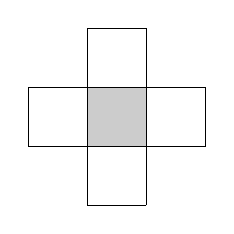
\begin{tikzpicture}
    \draw[step=0.75cm,black,thin] (0,0) grid (0.75,2.25);
    \draw[black,thin] (0.75,0.75) rectangle (1.5,1.5);
    \draw[black,thin] (-0.75,0.75) rectangle (0,1.5);
    \fill[gray!40, draw=black] (0,0.75) rectangle (0.75,1.5);

    \end{tikzpicture}

    \caption[The 4-neighbors representation of a pixel $p$]{The 4-neighbors representation of a pixel $p$. The pixel $p$ is centered on the grid with gray background. Source: adapted from~\citet{pedrini:08}.}
    \label{fig:n4-neighbors}
\end{figure}

Each pixel of the image is a unite distance from $(x, y)$. Some neighbors of $p$ might lie outside of the image boundaries if $(x, y)$ is on the border of the image \citep{gonzalez:02}. Those who will use neighborhood operations in the image might take this in consideration to avoid index out of range in those areas.

The four coordinates of the diagonals of $p$ are given by:
\begin{equation*}
    (x + 1, y + 1), (x + 1, y - 1), (x - 1, y + 1), (x - 1, y - 1)
    \label{eq:nd_neighbors}
\end{equation*}

This set of pixels are denoted by $N_D(p)$. When combined, the 4-\textit{neighbors} and $N_D(p)$ will generate the 8-\textit{neighbors} of $p$, known as $N_8(p)$ \citep{gonzalez:02}. Formally, we have:
\begin{equation*}
    N_8(p) = N_4(p) \cup N_D(p)
    \label{eq:n8_neighbors}
\end{equation*}

See figure~\ref{fig:n8-neighbors} for a reference on how the $N_8(p)$ neighborhood looks like.

\begin{figure}[ht]
    \centering
    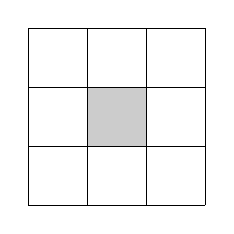
\begin{tikzpicture}
    \draw[step=0.75cm,black,thin] (0,0) grid (2.25,2.25);
    \fill[gray!40, draw=black] (0.75,0.75) rectangle (1.5,1.5);
    \end{tikzpicture}

    \caption[The 8-neighbors representation of a pixel $p$]{The 8-neighbors representation of a pixel $p$. The pixel $p$ is centered on the grid with gray background. Source: adapted from~\citet{pedrini:08}.}
    \label{fig:n8-neighbors}
\end{figure}

Despite these are the most common neighbors used in applications, other different distances from $p$ as well as connectivity can be applied. The idea of neighborhood can also be extended to 3-dimensional images where, instead of pixels, the voxels are the coordinates considered.


%% ------------------------------------------------------------------------- %%
\subsection{Connectivity}
\label{sec:connectivity}
Connectivity between pixels is a very important concept used to establish the boundaries of objects and regions in an image. To figure out if two pixels are connected, it must be determined if they are neighbors and if their gray levels satisfy some similarity criteria, such as gray levels, color or texture equality. For instance, in a binary image, where the pixels values vary in the range $[0, 1]$, two pixels may be 4-\textit{neighbors}, but they are connected if and only if they have the same value \citep{gonzalez:02}.


%% ------------------------------------------------------------------------- %%
\subsection{Arithmetic and logic operations}
\label{sec:ari_logic_operations}
Image arithmetic applies one of the standard arithmetic operations or a logical operator to two or more images. The operators are applied in a pixel-wise manner. In other words, the value of a pixel in the output image depends only on the values of the corresponding pixels in the input images. Hence, the images -- or the subsets, if is the case -- must be of the same size. Although image arithmetic is the most simple form of image processing, they are used extensively in a wide range of applications and its use can potentially produce very interesting practical results. A main advantage of arithmetic operators is that the process is very simple and therefore fast.

The most common arithmetic operations between two pixels, say $f_1(x, y)$ and $f_2(x, y)$ of two different images $f_1$ and $f_2$, are the addition, subtraction, multiplication and division as shown in table~\ref{tab:img_ari_operations} \citep{pedrini:08}.

\begin{table}[hb]
\centering
\begin{small}
\setlength{\tabcolsep}{12pt}
\renewcommand{\arraystretch}{1.75}

\begin{tabular}{|c|c|}\hline
 \thb{Name}     & \thb{Operation} \\ \hline
 Addition       & $f_1(x, y) + f_2(x, y)$ \\ \cline{1-2}
 Subtraction    & $f_1(x, y) - f_2(x, y)$ \\ \cline{1-2}
 Multiplication & $f_1(x, y) * f_2(x, y)$ \\ \cline{1-2}
 Division       & $f_1(x, y) / f_2(x, y)$ \\ \hline

\end{tabular}
\end{small}
\caption[Definition of addition, subtraction, multiplication and division arithmetic operations in two $f_1$ and $f_2$ images]{Definition of addition, subtraction, multiplication and division arithmetic operations in two $f_1$ and $f_2$ images. Source: adapted from~\citet{pedrini:08}.}
\label{tab:img_ari_operations}
\end{table}

Addition is used often for image averaging to reduce noise. Subtraction is used frequently for static background removal. Multiplication as well as division is applied to correct gray level shading~\citep{gonzalez:02}.

Once the arithmetic operations can potentially produce images with values out of the gray levels given in the original images, additional effort is frequently needed to work around this situation. For instance, when adding two images, some pixels of the resulting image may be greater than 255. Similarly, when subtracting two images, some pixels me be with negative values. One way to solve this issue is, after the arithmetic operation, perform a transformation in the gray levels of the resulting image to keep them within a suitable range~\citep{pedrini:08}.

Logic operations are also useful in computer vision and image processing applications. They are applied only in binary images, while arithmetic operations can be used with higher gray levels. The terminology adopted among authors and application developers is that pixels with zero value (black color) belongs to the objects while one value (white color) corresponds to the background. Table~\ref{tab:img_log_operations} shows how the logic operations can be computed~\citep{pedrini:08}.

\begin{table}[ht]
\centering
\begin{small}
\setlength{\tabcolsep}{12pt}
\renewcommand{\arraystretch}{1.75}

\begin{tabular}{|c|c|}\hline
 \thb{Name}     & \thb{Operation} \\ \hline
 AND    & $f_1(x, y)$ AND $f_2(x, y)$ \\ \cline{1-2}
 OR     & $f_1(x, y)$ OR $f_2(x, y)$ \\ \cline{1-2}
 XOR    & $f_1(x, y)$ XOR $f_2(x, y)$ \\ \cline{1-2}
 NOT    & NOT($f_1(x, y)$) \\ \hline

\end{tabular}
\end{small}
\caption[Definition of AND, OR, XOR and NOT logic operations in two $f_1$ and $f_2$ images]{Definition of AND, OR, XOR and NOT logic operations in two $f_1$ and $f_2$ images. Source: adapted from~\citet{pedrini:08}.}
\label{tab:img_log_operations}
\end{table}

The AND operation outputs 1 in the resulting image when both pixels, at same coordinates in the input images, are equal 1. XOR operation outputs 1 when only one of the pixels -- but not both -- has value 1; 0 otherwise. The result of OR operation is 1 when at least one of the pixels has 1 value. The NOT operation reverse the value of the pixel in the image \citep{pedrini:08}.

All the logic operators can be combined to create other more complex and robust operators. They can be used to combine information between images or to extract information of regions of interest from them~\citep{pedrini:08}.

In addition to the pixel-wise processing, logic and arithmetic operations can be used for neighborhood processing. Typically, this kind of processing uses masks, where terms such as windows and filters are often used as synonym of masks. The idea of the masks is to turn the value of the pixel a function of its own value and its neighbors. It is note mentioning that masks application are made under high computational cost. Therefore, they must be used carefully~\citep{pedrini:08}.


%% ------------------------------------------------------------------------- %%
\subsection{Image boundaries}
\label{sec:image_boundaries}

When working with neighborhood operations, the mask being used, independently of its size, can fall beyond the image boundaries. In other words, this means that, for an image $f$, with size $W \times H$, some part of the mask operator will be located in a nonexistent pixel from an index out of the range given by $W \times H$ matrix. Figure~\ref{fig:img_boundaries} shows an example of this phenomena in a $10 \times 8$ image being used as input for an 4-\textit{neighbors} operator.

\begin{figure}[ht]
    \centering
    \begin{tikzpicture}
    \draw[step=0.75cm,black,thin] (0,0) grid (7.5,6.0);
    \fill[pattern=north east lines, pattern color=blue, draw=black] (4.5,5.25) rectangle (5.25,6.0);
    \fill[pattern=north east lines, pattern color=blue, draw=black] (5.25,4.5) rectangle (6.0,5.25);
    \fill[pattern=north east lines, pattern color=blue, draw=black] (5.25,5.25) rectangle (6.0,6.0);
    \fill[pattern=north east lines, pattern color=blue, draw=black] (5.25,6.0) rectangle (6.0,6.75);
    \fill[pattern=north east lines, pattern color=blue, draw=black] (6.0,5.25) rectangle (6.75,6.0);
    \end{tikzpicture}

    \caption[Representation of an 4-\textit{neighbors} window mask going beyond image borders]{Representation of an 4-\textit{neighbors} window mask going beyond image borders. Here we can solve this problem, for instance ignoring the first and last lines and columns of the whole image during the operation. Source: adapted from~\citet{pedrini:08}.}
    \label{fig:img_boundaries}
\end{figure}

There are several ways to work around this problem. One simple mechanism is to simply ignore the pixels on the border where the mask go beyond. Despite this will avoid index out of bound errors, border pixels of the image will not be looked at. Another approach is to copy the corresponding pixels from the input image. Once again, the resulting image will have some not processed pixels in the border. Another strategy is to apply a different mask for the borders, which may consider the difference in the corners as well, to perform the operation, which can turn the operation more complex and computational costly~\citep{pedrini:08}.


%% ------------------------------------------------------------------------- %%
\section{Image histogram}
\label{sec:image_histogram}
In an image processing context, the histogram of an image normally refers to a histogram of the pixel intensity values. The most common representation is a graph or plot, which gives an overall idea about the intensity distribution of an image. The foundation of a histogram can be seen as a set of bins, where each bin is representing a certain intensity value from a given range. A simple algorithm to compute a histogram of an image may examines all pixels in the image and assigns each to a bin depending on the pixel intensity. In the end, each bin will have the number of pixels of its own intensity value \citep{gonzalez:02}.

For instance, in an 8-bit grayscale image there are 256 different possible intensities, and so the histogram will graphically display 256 numbers showing the counting of occurrences of those grayscale values. It is also possible to compute histograms of color images. In this particular case, the channels of the color space in use are split individually from where a separate histogram is calculated.

\begin{figure}[H]
    \centering
    \begin{subfigure}[t]{0.4\textwidth}
        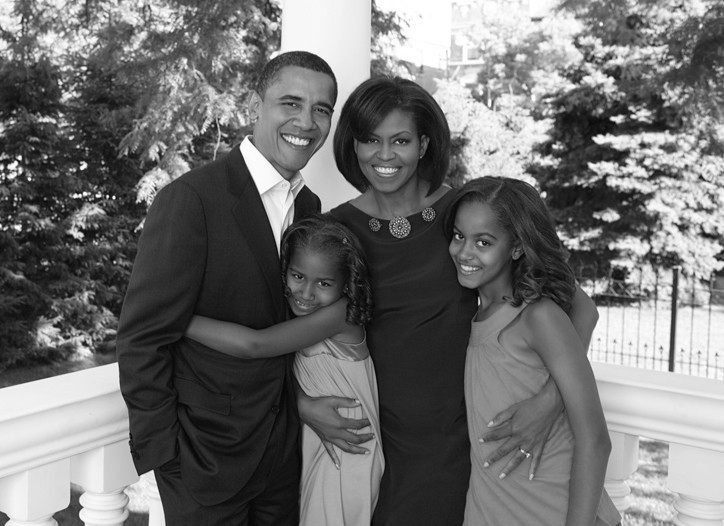
\includegraphics[width=\textwidth]{obama_gs}
    \end{subfigure}
    ~
    \begin{subfigure}[t]{0.54\textwidth}
        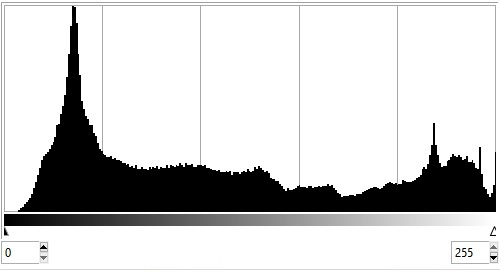
\includegraphics[width=\textwidth]{obama_histogram}
    \end{subfigure}
    \caption[Grayscale image with its respective histogram]{Grayscale image with its respective histogram. Left image is a sample from Pratheepan dataset, transformed to grayscale. On the right we have its histogram of pixel intensity values in the range [0, 255].}
    \label{fig:obama_hist}
\end{figure}

A histogram can be seen as a probability distribution, once the number of pixels for a given intensity level gives an estimate of the probability of occurrence of this intensity level~\citep{gonzalez:02}. Several statistical measures can be obtained from a histogram such that minimum and maximum values, mean, median, standard deviation, and percentiles \citep{pedrini:08}. Those measures as well as the histogram itself are fundamental for the methods described in chapter~\ref{cap:proposed-solution} of the proposed solution.


%% ------------------------------------------------------------------------- %%
\section{Image segmentation}
\label{sec:image_segmentation}
Image segmentation refers to partitioning an image into different regions that are homogeneous with respect to some image feature~\citep{gonzalez:02}. Those regions, or objects, are the fundamental parts of an image. With respect to the human visual perception, humans use their visual sense to effortlessly partition their surrounding environment into different objects to help themselves to recognize them, guide their movements, and for almost every other task in their lives~\citep{konstantinos:00}.

Segmentation of complex images is one of the most difficult tasks in the field of image processing, where the accuracy determines whether a successful operation or not~\citep{gonzalez:02}. It is a heavy process that includes many interacting components that are involved with the analysis of color, shape, motion, and texture of objects in images. Despite the segmentation of images is a natural activity for the human visual system, it is definitely not easy to create algorithms whose performance is comparable to that of the human visual system~\citep{konstantinos:00}.

Image segmentation is usually the first task of any image analysis process. All subsequent tasks, such as feature extraction and object recognition rely heavily on the quality of the segmentation~\citep{konstantinos:00}. The algorithms created for image segmentation generally are based on one of two basic properties of intensity values: \emph{discontinuity}, where abrupt changes in intensity, such as points, lines, and edges are detected, and \emph{similarity}, whose approaches are based on regions partitioning, according to a set of predefined criteria~\citep{gonzalez:02}.

One of the \emph{similarity} methods it is the thresholding: a popular and clever method used to segment regions of an image, especially in applications where speed is an important factor -- that is the case for skin detection, once it is used, in general, for face detection, gesture analysis, face tracking, video surveillance systems, medical image analysis, and other human-related image processing applications. Due the simplicity of implementation, several authors apply this technique on skin detection task~\citep{kovac:03, chai:99, basilio:11, kaur:12, shaik:15, kumar:15}. Others extend this application by using adaptive thresholding~\citep{yogarajah:11, tan:12}.

The method proposed by~\citet{brancati:17}, where a set of dynamic correlation rules are computed to determine skin pixels can be classified as the kind of \emph{similarity} method. Subsequently, our proposed enhancements described in chapter~\ref{cap:proposed-solution}, in a pixel-based manner, is also of this kind. For that reason, a brief introduction on thresholding will be given in section~\ref{sec:thresholding}.


%% ------------------------------------------------------------------------- %%
\subsection{Thresholding}
\label{sec:thresholding}


%% ------------------------------------------------------------------------- %%
\section{Color models}
\label{sec:color_models}

The use of color images in computer vision or image processing can be motivated by two main factors. The first refers to the powerful characteristic of color to function as a descriptor that often simplifies the identification and extraction of an object in a scene. The second is related to the ability of humans to discern thousands of tonalities and intensities compared to only a few dozen levels of gray \citep{gonzalez:02}.

The visual perception of color by the human eye should not vary according to the spectral distribution of the natural light incident upon an object. In other words, the color appearance of objects remains stable under different lighting conditions. This phenomenon is known as color constancy \citep{gevers:12}.

As an example, the grass of a soccer stadium remains green throughout the day, even at dusk when, from a physical point of view, sunlight has a more reddish appearance.

The human perception of colors occurs by the activation of nerve cells that send signals to the brain about brightness, hue and saturation, which are usually the features used to distinguish one color from another \citep{gonzalez:02}.

The brightness gives the notion of chromatic intensity. Hue represents the dominant color perceived by an observer. Saturation refers to the relative purity or amount of white light applied to the hue. Combined, hue and saturation are known as chromaticity and, therefore, a color must be characterized by its brightness and chromaticity \citep{gonzalez:02}.

Colors can be specified by mathematical models in tuples of numbers in a coordinate system and a subspace within that system where each color is represented by a single point. Such models are known as the color models \citep{gonzalez:02}.

These models can be classified as of two types: the additive models in which the primary color intensities are added to produce other colors and subtractive, where colors are generated by subtracting the length of the dominant wave from the white light.

The following sections briefly describe some of the major color models, as well as their variants and main areas of application.

%% ------------------------------------------------------------------------- %%
\subsection{Munsell color model}
\label{sec:modelo_cores_munsell}

Pioneer in an attempt to organize the perception of color in a color space, Albert H. Munsell was able to combine the art and science of colors in a single theory \citep{konstantinos:00}.

The principle of equality of visual spacing between the components of the model is the essential idea of the Munsell color model. These components are hue, value, corresponding to luminance, and chroma, corresponding to saturation \citep{konstantinos:00}.

The model is represented by a cylindrical shape and it can be seen in the figure ~\ref{fig:munsell-system}. The hue is arranged in the circular axis consisting of five base as well as five secondary colors, the saturation in the radial axis and the luminance in the vertical axis in a range varying from 0 to 10.

\begin{figure}[!ht]
  \centering
  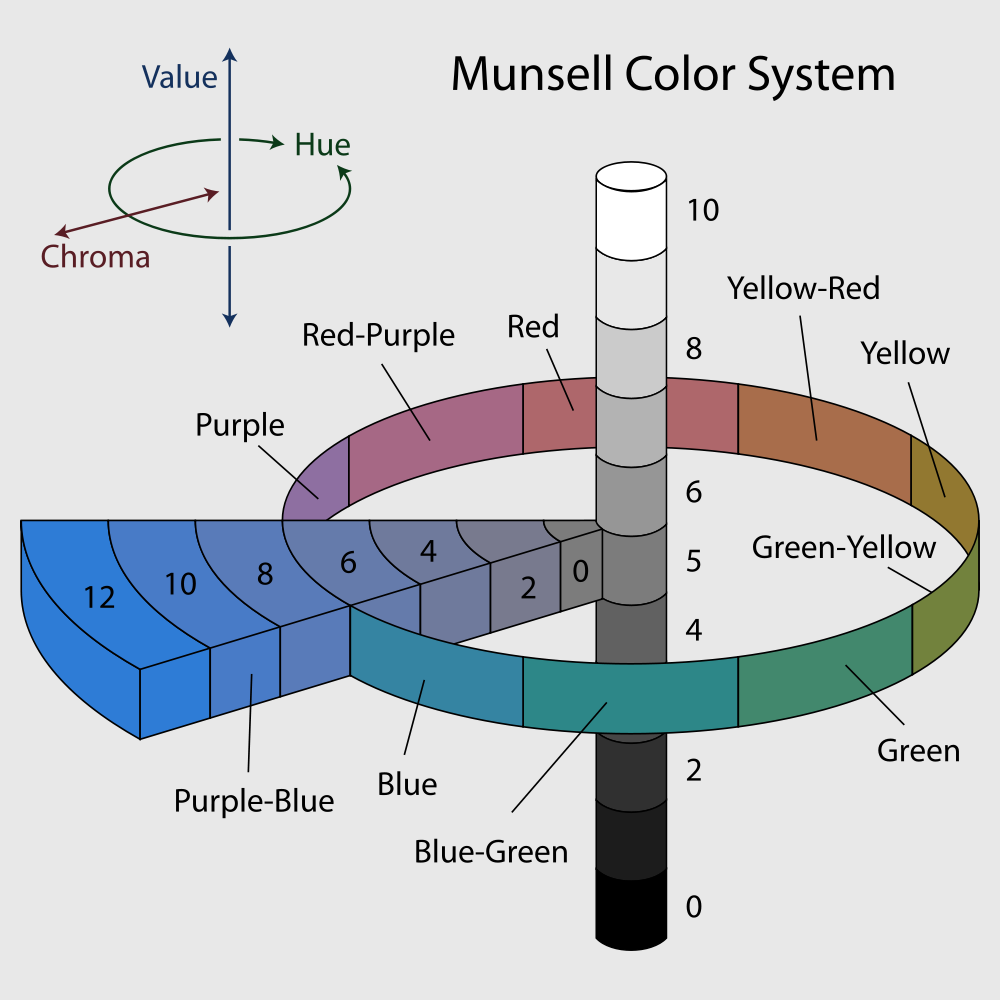
\includegraphics[width=.55\textwidth]{munsell-system}
  % fonte https://commons.wikimedia.org/wiki/File:Munsell-system.svg
  \caption[Munsell color model.]{Munsell color model represented by a cylindrical shape. The hue is arranged on the circular axis consisting of five base and five secondary colors, the saturation on the radial axis and the luminance on the vertical axis in a range varying from 0 to 10. Source: \citet{rus:07}.}
  \label{fig:munsell-system} 
\end{figure}

%% ------------------------------------------------------------------------- %%
\subsection{CIE color model}
\label{sec:modelo_cores_cie}

In 1931, the CIE established the first mathematical model of color numerical specification, whose objective was to analyze the relationship between the physical aspects of colors in the electromagnetic spectrum and their perception by the human visual system to determine how an ordinary person perceives the color. A review of this specification was published in 1964 \citep{gonzalez:02}.

The experiment that originated the standard consisted in detecting the colors perceived by an observer from a mixture of three primary colors X, Y and Z called tristimulus values. These coordinates gave rise to the CIE XYZ color space which encompasses all the colors that can be perceived by an ordinary human being. For this reason, it is considered an device independent representation \citep{konstantinos:00}.

The system proposed by the CIE XYZ to describe a color is based on a luminance component Y, and two additional components X and Z, that bring the chromaticity information. This system is formed by imaginary colors that can be expressed as combinations of the normalized measures shown in the equations~\ref{eq:cie_x}, \ref{eq:cie_y} and \ref{eq:cie_z}.

\begin{equation}
  x = \frac{X}{X + Y + Z}
\label{eq:cie_x}
\end{equation}

\begin{equation}
  y = \frac{Y}{X + Y + Z}
\label{eq:cie_y}
\end{equation}

\begin{equation}
  z = \frac{Z}{X + Y + Z}
\label{eq:cie_z}
\end{equation}

where $x + y+ z = 1$.

Combinations of negative values and other problems related to selecting a set of real primaries are eliminated. The chromaticity coordinates $x$ and $y$ allow to represent all colors in a two-dimensional plane, also known as a chromaticity diagram, which can be seen in the figure ~\ref{fig:cie-cromaticity-diagram}.

\begin{figure}[!ht]
  \centering
  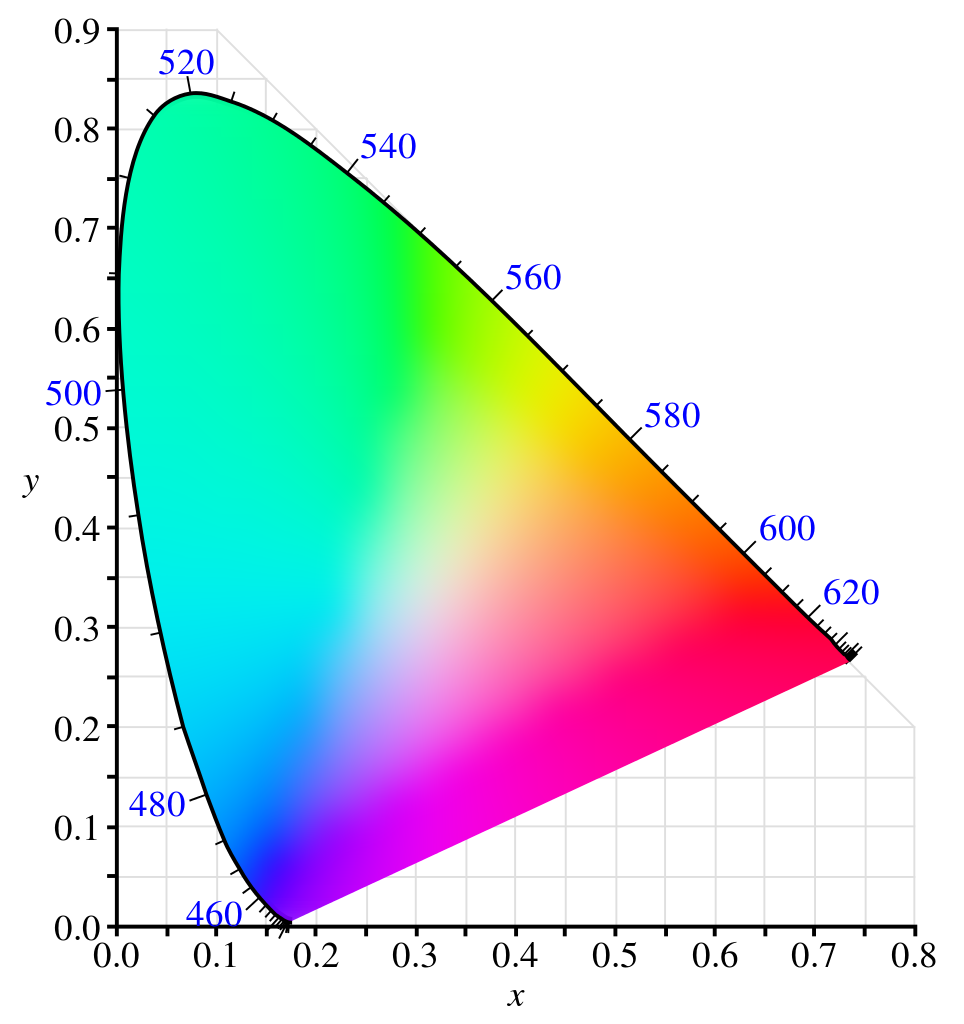
\includegraphics[width=.5\textwidth]{cie-cromaticity-diagram}
  % fonte https://en.wikipedia.org/wiki/File:CIE1931xy_blank.svg
  \caption[CIE 1931 chromaticity diagram]{CIE 1931 chromaticity diagram. The points representing pure colors in the electromagnetic spectrum are labeled according to their wavelengths and are located along the curve from the right end of the x-axis, corresponding to the red color, to the left end of the same axis, corresponding to the violet color, forming a polygon similar to a horseshoe. The internal points correspond to all possible combinations of visible colors. Source: \citet{ben:09}.}
  \label{fig:cie-cromaticity-diagram} 
\end{figure}

The coordinates $ (x = 1/3, y = 1/3) $ correspond to the location of white light, also known as white point, and serve as reference in the process of image capture, coding, or reproduction.

CIE also derived and standardized two other color models based on CIE XYZ specification and, likewise, are device independent. Both are perceptually uniform, which means that equal perceptual distances separate all colors in the system~\citep{vezhnevets:03}. As an example, the gray scale of the space should allow for a smooth transition between black and white.

The first one was designed to reduce the problem of perceptual non-uniformity. Some Uniform Chromaticity Scale (UCS) diagrams were proposed based on mathematical equations to transform the values XYZ or the coordinates $x, y$ into a new set of values $(u, v)$, which gave rise to the 1960 CIE $uv$ chromaticity diagram~\citep{gevers:12}.

Still with unsatisfactory results, the CIE made a new change by multiplying the $v$ component by a factor of 1.5. In addition, the brightness scale given by the Y component has been replaced by $L^* = [0, 100]$ to better represent the differences in luminosity that are equivalent. This revision originated the CIE 1976 $L^*u^*v^*$ color model, commonly known by the acronym CIELuv~\citep{gevers:12}.

In 1976 the CIE adopted a new color model, based on the $L, a, b$ model, proposed by Richard Hunter in 1948, which best represented the uniform spacing of colors. Named CIE $L^*a^*b^*$ and known by the acronym CIELab, it is a space based on opponent colors \footnote{Theory started around 1500 when Leonardo da Vinci concluded that colors are produced by mixing yellow and blue, green and red, and white and black. In 1950, this theory was confirmed when optically-colored signals were detected at the optical connection between the retina and the brain~\citep{gevers:12}.} in which the color stimuli of retina is converted to distinctions between light and dark, red and green, and blue and yellow, represented by the axes $L^*$, $a^*$, and $b^*$, respectively~\citep{gevers:12}.


%% ------------------------------------------------------------------------- %%
\subsection{RGB color model}
\label{sec:modelo_cores_rgb}

The RGB model, an acronym for Red, Green, and Blue, is an additive color model in which the three primary colors red, green and blue are added to produce the others \citep{gonzalez:02}.

This system was based on the trichromatic theory of Thomas Young and Hermann Helmholtz in the mid-19th century and can be represented graphically
through the unit cube defined on the axes R, G and B, as illustrated in the figure~\ref{fig:rgb-cube} \citep{konstantinos:00}.

\begin{figure}[!ht]
  \centering
  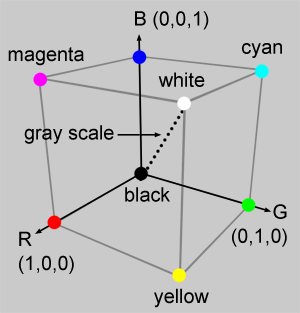
\includegraphics[width=.35\textwidth]{rgb-cube}
  % http://www.scratchapixel.com/old/lessons/3d-basic-lessons/lesson-5-colors-and-digital-images/color-spaces/
  \caption[Unit cube representing the colors of the RGB model]{Unit cube representing the colors of the RGB model. The origin, given by the vertex $(0, 0, 0)$, represents the black color. The vertex $(1, 1, 1)$, opposite the origin, represents the white color. The highlighted vertices on the axes represent the primary colors and the others are the complement of each. Each point inside the cube corresponds to a color that can be represented by the triple $(r, g, b)$, where $r, g, b \in [0, 1]$. The shades of gray are represented along the main diagonal of the cube, with each point along this diagonal being formed by equal contributions of each primary color. Source: adapted from \citet{gonzalez:02}.}
  \label{fig:rgb-cube} 
\end{figure}

It is noteworthy that there are two ways of representing the RGB space: linear and non-linear. The above-mentioned system shows the non-linear model, whose abbreviation is $R'G'B'$, and is most used by devices and applications because of their similarity to the human visual system. In the literature, this system is frequently cited with the acronym RGB, which makes the nomenclature dubious, since the linear model is also called RGB and, therefore, the conversion between color spaces must be done with some caution. It is also important to note that linear RGB values are rarely used to represent an image since they are perceptually highly non-uniform \citep{konstantinos:00}.


%% ------------------------------------------------------------------------- %%
\subsection{CMY color model}
\label{sec:modelo_cores_cmy}

The CMY model is based on the complementary primary colors Cyan, Magenta, and Yellow and, unlike RGB, is a subtractive color model in which colors are generated by subtracting the length of the dominant wave from the white light and, therefore, the resulting color corresponds to the light that is reflected \citep{gonzalez:02}.

One way to get the CMY system is:\\
\begin{equation}
  \begin{bmatrix}
    C \\ M \\ Y
  \end{bmatrix} = 
  \begin{bmatrix}
    B \\ R \\ R
  \end{bmatrix} +
  \begin{bmatrix}
    G \\ B \\ G
  \end{bmatrix}
\end{equation}

\noindent or by making a change of coordinates by subtracting the primary colors R, G and B of the white color $W = (1, 1, 1)$ \citep{gonzalez:02}:
\begin{equation}
  \begin{bmatrix}
    C \\ M \\ Y
  \end{bmatrix} = 
  \begin{bmatrix}
    1 \\ 1 \\ 1
  \end{bmatrix} -
  \begin{bmatrix}
    R \\ G \\ B
  \end{bmatrix}
\end{equation}

Likely RGB, CMY is device dependent. The model is widely used in equipment that deposits colored pigments on paper, such as color printers or photocopiers. The figure~\ref{fig:cmy-model} shows how the model components are combined to generate the other colors.

\begin{figure}[!ht]
  \centering
  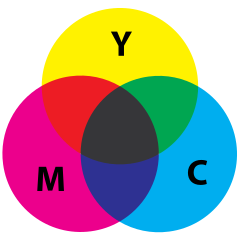
\includegraphics[width=.25\textwidth]{cmy-model}
  % https://en.wikipedia.org/wiki/File:SubtractiveColor.svg
  \caption[CMY subtractive color model]{CMY subtractive color model. It is interesting to note that the intersection of yellow with magenta generates the red color, magenta with cyan generates the blue color and cyan with yellow generates the green color. Source: \citet{rus:08}.}
  \label{fig:cmy-model}
\end{figure}

Overlapping the CMY primary colors in equal amounts to generate the black color typically creates a tint that is close to brown or dark green. To avoid this undesired effect, the black component is usually added to the system, represented by the letter K. This operation gives rise to a new model known as \textbf{CMYK}~\citep{gonzalez:02}.

%% ------------------------------------------------------------------------- %%
\subsection{Color models of the YUV family}
\label{sec:modelo_cores_yuv}

Color models of this family is also known as orthogonal color spaces. They are able to reduce the redundancy present in RGB color channels and represent the color with statistically independent components - as independent as possible \citep{kakumanu:07}.

The acronym YUV stands to a set of color spaces of which the luminance information, represented by the Y component, is coded separately from the chrominance, given by the components U and V. The components U and V are representations of signals of the difference of the blue subtracted from luminance (B-Y) and red subtracted from luminance (R-Y). It is used to represent colors in analogue television transmission systems in the Phase Alternating Line (PAL) and Sequential Color with Memory (SECAM)~\citep{pedrini:08}.

The transformation of the RGB space to YUV is given by:\\
\begin{equation}
  \begin{bmatrix}
    Y \\ U \\ V
  \end{bmatrix} = 
  \begin{bmatrix}
     0.299 &  0.587 &  0.114 \\
    -0.147 & -0.289 &  0.436 \\
     0.615 & -0.515 & -0.100 \\
  \end{bmatrix}
  \begin{bmatrix}
    R \\ G \\ B
  \end{bmatrix}
\end{equation}
where $0 \leq R, G, B \leq 1$.

Analogous to the YUV, the YIQ model was adopted in 1950 by the National Television System Committee (NTSC), an American standard for color television signal transmission. In this model, the Y component corresponds to luminance and the components I (hue) and Q (saturation) encode the chrominance information \citep{pedrini:08}.

The transformation of the RGB space to YIQ is given by:\\
\begin{equation}
  \begin{bmatrix}
    Y \\ I \\ Q
  \end{bmatrix} = 
  \begin{bmatrix}
    0.299  &  0.587 &  0.114 \\
    0.596  & -0.275 & -0.321 \\
    0.212  & -0.523 & -0.311 \\
  \end{bmatrix}
  \begin{bmatrix}
    R \\ G \\ B
  \end{bmatrix}
\end{equation}
where $0 \leq R, G, B \leq 1$.

Another color model of the YUV family is the YCbCr, mathematically defined by a coordinate transformation with respect to some RGB space~\citep{pedrini:08}.

The YCbCr model is widely used in digital videos. In this system, the Y component represents luminance, computed as a weighted sum of RGB values. Cb component gives the measurement of the difference between the blue color and a reference value, similar to the Cr component which is the measurement of the difference between the red color and a reference value~\citep{pedrini:08}.

The transformation of the RGB space to YCbCr is given by:\\
\begin{equation}
  \begin{bmatrix}
    Y \\ Cb \\ Cr
  \end{bmatrix} = 
  \begin{bmatrix}
     0.299 &  0.587 &  0.114 \\
    -0.169 & -0.331 &  0.5   \\
     0.5   & -0.419 & -0.081 \\
  \end{bmatrix}
  \begin{bmatrix}
    R \\ G \\ B
  \end{bmatrix}
\end{equation}


%% ------------------------------------------------------------------------- %%
\subsection{Color models of the HSI family}
\label{sec:modelo_cores_hsi}

Hue, Saturation, and Intensity (HSI) models are best suited for image processing applications from the user's point of view, due the correlation with human perception of the color\citep{konstantinos:00}.

In this model, as in YIQ, the intensity given by I component is decomposed from the chrominance information, represented by the hue (H) and saturation (S) \citep{konstantinos:00}. The combination of these components results in a pyramidal structure which can be seen in figure~\ref{fig:hsi-model}.

\begin{figure}[!ht]
  \centering
  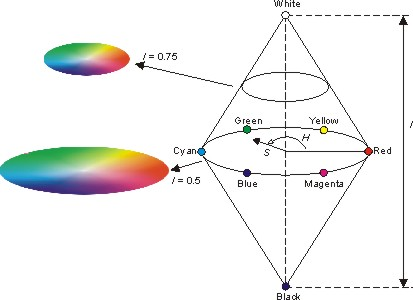
\includegraphics[width=.7\textwidth]{hsi-model}
  % http://www.blackice.com/images/HSIColorModel.jpg
  \caption[Graphical representation of the HSI model]{Graphical representation of the HSI model. The hue describes the color itself, in the form of an angle $\theta$, where $\theta \in [0, 360]$. Red is at 0 degree, yellow at 60, green at 120, and so on. The saturation component, which varies between 0 and 1, indicates how much color is polluted with white color. The intensity scale is between $[0, 1]$, where 0 means black and 1, white. Source: \citet{blackice:16}.}
  \label{fig:hsi-model} 
\end{figure}

The transformation of the components of the RGB space to HSI is given by the equations:
\begin{align}
\label{eq:rgb_para_hsi}
\begin{split}
  \theta &= cos^{-1} \bigg( \frac{(R - G) + (R - B)}{2 \sqrt{(R - G)^2 + (R - B)(G - B)}} \bigg)
  \\[0.5em]
  H &= \begin{cases}
            \theta,       & \text{if}\ B \leq G\\
            360 - \theta, & \text{otherwise}\\
       \end{cases}
  \\[0.5em]
  S &= 1 - \frac{3 min(R, G, B)}{R + G + B}
  \\[0.5em]
  I &= \frac{R + G + B}{3}
\end{split}
\end{align}

It is important to note that the values R, G and B must be normalized in the interval between 0 and 1. The intensity $I$ and the saturation $S$ are also normalized between 0 and 1.

Another model of this family is formed by the components Hue, Saturation and Value (HSV) and its three-dimensional graphical representation is a hexagonal pyramid derived from the RGB cube \citep{pedrini:08}. Value, in this context, is the luminance component.

The various hue shades are represented at the top of the pyramid, the saturation is measured along the horizontal axis and value is measured along the vertical axis, which passes through the center of the pyramid. The hue, which corresponds to the edges around the vertical axis, varies from 0 (red) to 360 degrees and the angle between the vertices is 60 degrees. The saturation varies from 0 to 1 and is represented as the ratio of the purity of a given hue to its maximum purity, that is, when $S = 1$. Value varies from 0, at the peak of the pyramid representing the black color, to 1 at the base, where the intensities of the colors are maximum~\citep{pedrini:08}.

The transformation of the components of the RGB space to HSV is given by the equations:
\begin{align}
\label{eq:rgb_para_hsv}
\begin{split}
  H &=  \begin{cases}
            60\ffrac{(G - B)}{M - m}, & \text{if}\ M = R\\[0.7em]
            60\ffrac{(B - R)}{M - m} + 120, & \text{if}\ M = G\\[0.7em]
            60\ffrac{(R - G)}{M - m} + 240, & \text{if}\ M = B
       \end{cases}
  \\[0.5em]
  S &=  \begin{cases}
            \ffrac{(M - m)}{M}, \quad &\text{if}\ M \neq 0\\[0.7em]
            0, \quad &\text{otherwise}\\
       \end{cases}
  \\[0.5em]
  V &= M
\end{split}
\end{align}

\noindent where $m = min(R, G ,B)$ and $M = max(R, G ,B)$. The luminance $V$ and saturation $S$ are normalized between 0 and 1. The $H$ hue ranges from 0 to 360 degrees.

Similarly to HSV, the Hue, Saturation and Lightness (HSL) model is a three-dimensional representation and is formed by two cones of height 1, whose bases are coincident \citep{pedrini:08}.

The hue is determined by the points in the circle of the common bases to the cones. The saturation varies from 0 to 1, depending on the distance to the axis of the cone. The lightness is along the vertical axis common to the two cones and varies in the scale $[0, 1]$, where 0 means black and 1, white \citep{pedrini:08}.

The conversion of the RGB space to HSL is given by the equations:
\begin{align}
\label{eq:rgb_para_hsl}
\begin{split}
  H &=  \begin{cases}
            60\ffrac{(G - B)}{M - m}, & \text{if}\ M = R\\[0.7em]
            60\ffrac{(B - R)}{M - m} + 120, & \text{if}\ M = G\\[0.7em]
            60\ffrac{(R - G)}{M - m} + 240, & \text{if}\ M = B
       \end{cases}
  \\[0.5em]
  S &=  \begin{cases}
            \ffrac{(M - m)}{M + m}, & \text{if}\ 0 < L \leq 0,5\\[0.7em]
            \ffrac{(M - m)}{2 - (M + m)}, & \text{if}\ L > 0,5\\[0.5em]
            0, & \text{if}\ M = m\\
       \end{cases}
  \\[0.5em]
  L &= \frac{M + m}{2}
\end{split}
\end{align}

\noindent where $m = min(R, G ,B)$ and $M = max(R, G ,B)$. The lightness $V$ and saturation $S$ are normalized between 0 and 1. Note that the transformation of the $H$ component is the same as that used in the conversion of the RGB to HSV space in \ref{eq:rgb_para_hsv} and varies between 0 and 360 degrees.

All the color models of this family have the property of thinking of lighter colors, obtained by increasing the brightness or lightness, and darker colors, by the diminution of the same values. The intermediate colors are produced by decreasing the saturation~\citep{pedrini:08}.